
\section{Beugró gyüjtemények}

\subsection{UML Állapotgép}

	\begin{enumerate}
		\item Állapottábla felírása állapotgépből.

		\item Állapotgép alapján állítások eldöntése

			PL:

				\begin{center}
					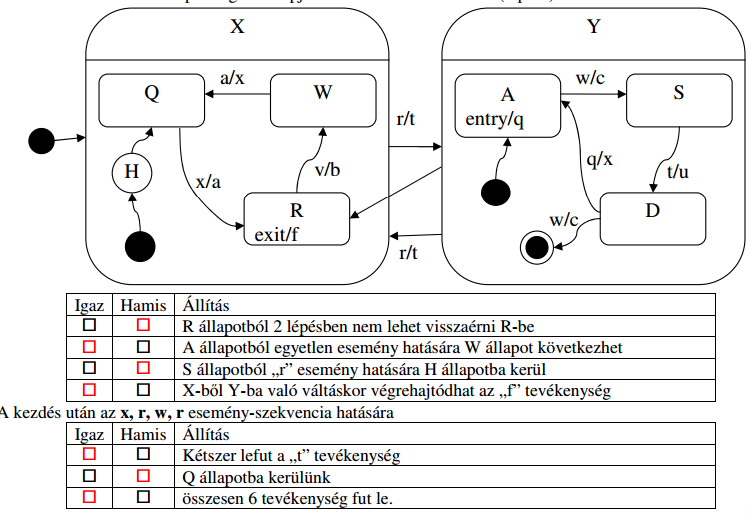
\includegraphics[scale=0.7]{img/table5}
				\end{center}
	\end{enumerate}

\subsection{Magic UML igaz hamis Osztálydiagramból}

	Hányszor fordult elő: 8/10
\subsection{Elmélet}

	\begin{enumerate}

		\item A szoftver fejlesztési folyamat ICOM modelljében mik a vezérlések/kényszerek (control/constraints)? (3pont)

			\begin{enumerate}
				\item Budget
				\item Schedule
				\item Standards

				\begin{center}
					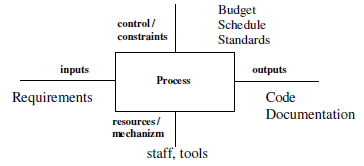
\includegraphics[scale=0.7]{img/icom}
				\end{center}
			\end{enumerate}

		\item Sorolja fel a tesztelés során végrehajtandó kiértékelési (evaluation) folyamatnak a bemeneteit.

			\begin{enumerate}
				\item test results
				\item expected results
			\end{enumerate}
			\begin{center}
			    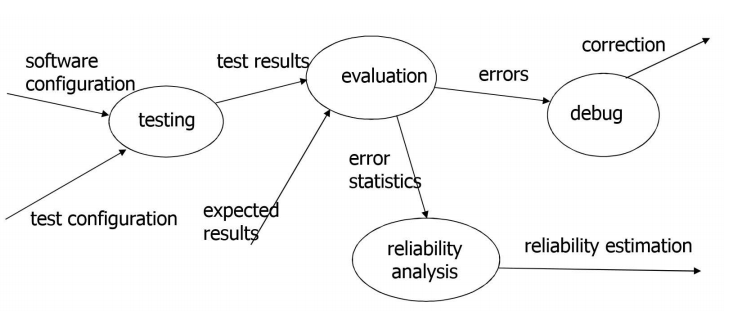
\includegraphics[width=0.60\textwidth]{img/evaluation}
			 \end{center}

		\item	Scrum agilis módszertan futamának

			\begin{enumerate}
				\item Bemenet: Sprint backlog
				\item Kimenet: Working increment of the software
				\item időbeli hossz: ~30 days
			\end{enumerate}

		\item Jelőlje be hogy az egyes szerődéses feltételek megszegse esetén melyik oldal a hibás!(3 pont)

				\begin{center}
					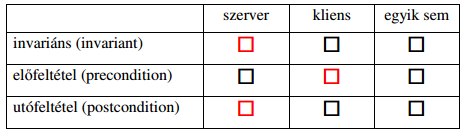
\includegraphics[scale=0.7]{img/table1}
				\end{center}

			\small \textit{Egyszerű megjegyzés érdekében, az előfeltétel vonatkozik csak a kliensre} \normalsize

		\item Az alábbi táblázatban adja meg a Rational Unified Process (RUP) fő munkafolyamatait é snevezze meg a hozzá tartozó nétezz.

				\begin{center}
					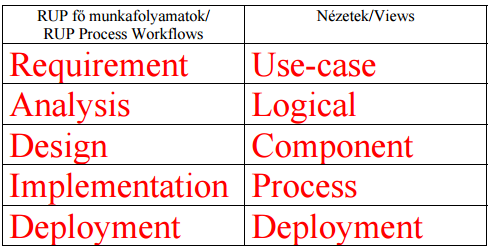
\includegraphics[scale=0.7]{img/table2}
				\end{center}

	\item Mit jelent a CMM?

		Capability Maturity Model

	\item Jelölje meg az igaz állításokat:

				\begin{center}
					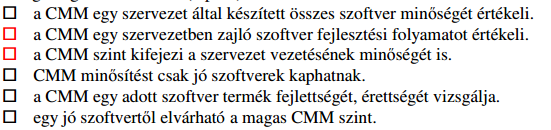
\includegraphics[scale=0.7]{img/table3}
				\end{center}

	\item Adott az alábbi use-case diagram részlet. Jelölje be az igaz állítást!

				\begin{center}
					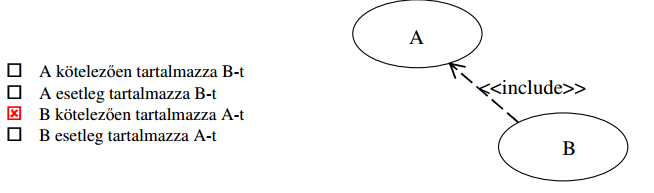
\includegraphics[scale=0.7]{img/table4}
				\end{center}

	\item Követelmény specifikálásakor a leíráson kívül milyen lényeges információt kell még rögzíteni?(3 pont)

		Azonosító, forrás, Ellenörzés módja

	\item Az Extrém Programozás (XP) projektet írja le az alábbi (hiányos) ábra. Adja meg azoknak az elemeknek a számát és nevét, amelyek a Rational Unified Process (RUP) alapelveihez közvetlenól kapcsolódnak.

		\begin{center}
			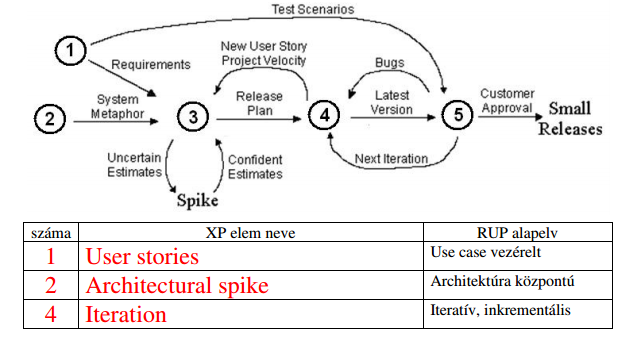
\includegraphics[scale=0.7]{img/table6}
		\end{center}

	\item Jelölje meg, hogy a Scrum módszertanban kik tartoznak a csirkék (chickens, ancillary roles) közé! (2pont)

		\begin{center}
			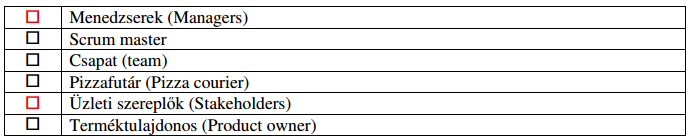
\includegraphics[scale=0.7]{img/table7}
		\end{center}

	\item Adja meg, hogy a jelölt elemek melyik UML meta-modell elemek példánya!

		\begin{center}
			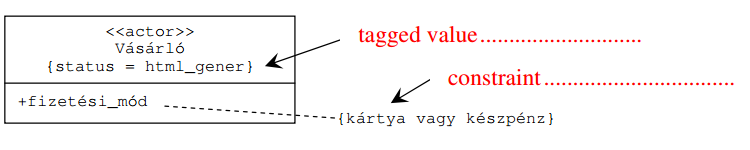
\includegraphics[scale=0.7]{img/table8}
		\end{center}

	\item Az Agilis Kiáltván ( "Agile Manifesto") a klasszikus fejlesztés hagyományos fogalmait újakra cseréli. Mik az új fogalmak? ( 4pont)

		\begin{center}
			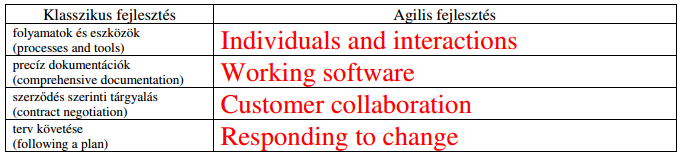
\includegraphics[scale=0.7]{img/table9}
		\end{center}

	\item Adott a következő BNF specifikáció

		\begin{center}
			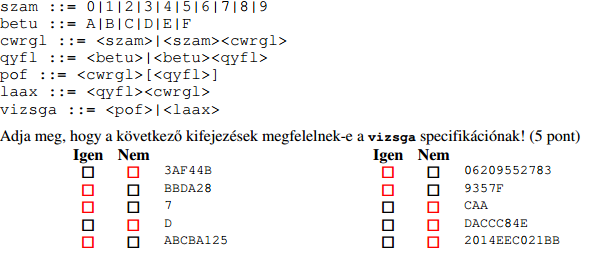
\includegraphics[scale=0.7]{img/table10}
		\end{center}

	\item Mi az A és B az UML diagramon?

		\begin{center}
			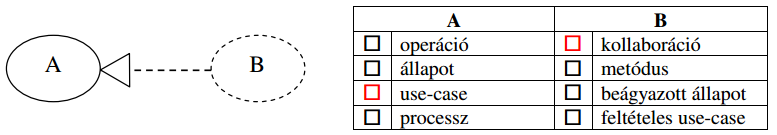
\includegraphics[scale=0.7]{img/table11}
		\end{center}

	\item Egy objektum metódusa szekvenciálisan kohézív, ha a metódus:

		\begin{center}
			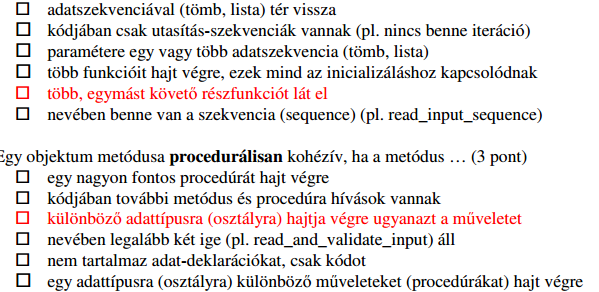
\includegraphics[scale=0.7]{img/table12}
		\end{center}

	\item Jelölje az állítások mellet 1-5-ig , hogy minimáisan melyik CMM szinttől igazak! Ha az állítás nem értelmezhető, akkor tegyen X-et! (4pont)

		\begin{center}
			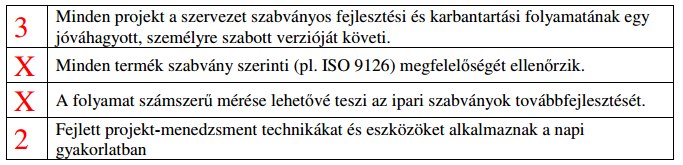
\includegraphics[scale=0.7]{img/table13}
		\end{center}

		\begin{center}
			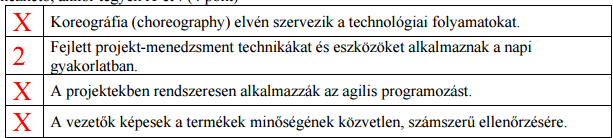
\includegraphics[scale=0.7]{img/table22}
		\end{center}

	\item Rajzolja e az alábbi UML2 diagramba a hiányzó kapcsolatokat! (3 pont)

		\begin{center}
			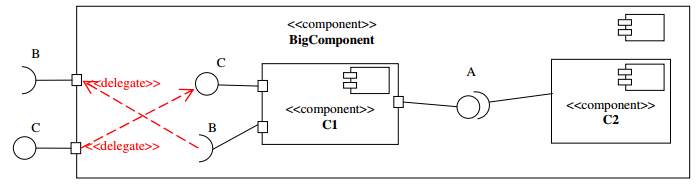
\includegraphics[scale=0.7]{img/table14}
		\end{center}

	\item Subversion-ben a commit (check in) végrehajtása attól függ, hogy az utolsó letöltés ( check out/update) óta módosult-e a letöltött és/vagy a repositoryban tárolt változat.

		\begin{center}
			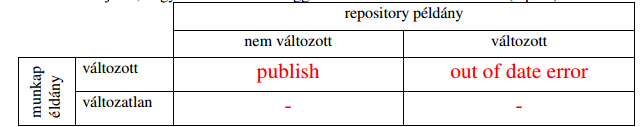
\includegraphics[scale=0.7]{img/table15}
		\end{center}

	\item Milyen általánosan kiterjesztő technikákat ( general extension mechanisms) alkalmaz az UML2? (3pont)

		Constraint, Stereotype, tagged value

	\item Mi a Rational Unified Proess (RUP) életciklus modelljének utlsó fázisa? Milyen tevékenységek tartoznak ebbe a fázisba:

	Utolsó fázis: \textit{Transition}

	tevékenységek: \textit{Manufacturing, delivering, training}

	\item Egy UML2 modelben legyen egy Student osztályunk. Daniel a Student osztály valós idejű példányának UML2-beli modellje.

		\begin{center}
			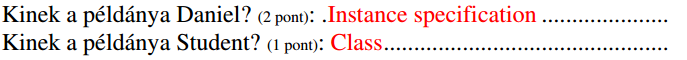
\includegraphics[scale=0.7]{img/table16}
		\end{center}

	\item Mik a hasonlóságok az adafolyam (DFD) és a use-case ( UC) modellek között? ( 3pont)

		\begin{enumerate}
			\item Funkcionalitást írnak le
			\item terminátor - actor
			\item folyamat ( process) - use-case
		\end{enumerate}

	\item Sorolja fel a Rational Unified Process ( RUP) életciklus modelljében szereplő "támogató munkafolyamatokat" (supporting workflows)! (3 pont)

		konfigurációs menedzsment, menedzsment, környezet

	\item A specikikáció célja a követelményeknek eleget tevő rendszer formális leírása. Milyen három fontos nézőpontból készítjük a leírásokat? (3 pont)

		\begin{enumerate}
			\item Funkcionalitás
			\item Szerkezet ( struktúra )
			\item dinamika ( viselkedés )
		\end{enumerate}

	\item Mik a konfigurációs menedzsment fő folyamatai? (4 pont)

		\begin{enumerate}
			\item Storage Configuration Items
			\item Build Management
			\item Change Management
			\item Relase Management
		\end{enumerate}

	\item Minek az ellenörzésére irányulnak az alábbi tesztelések? (4 pont)

		\begin{center}
			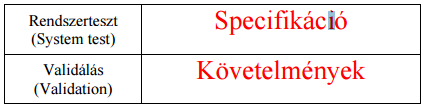
\includegraphics[scale=0.7]{img/table17}
		\end{center}

	\item Az UML2 Activity diagram egy másik UML2 diagram speciális esetének tekinthető. Melyik ez a diagram? Hasonlítsa össze a két diagramot!

		\begin{center}
			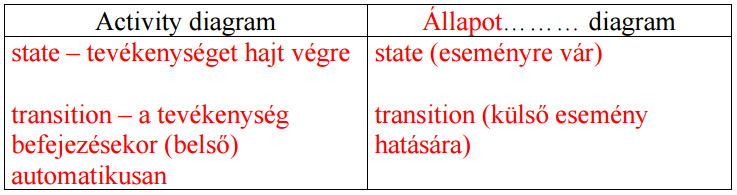
\includegraphics[scale=0.7]{img/table18}
		\end{center}

	\item Mi történik refaktoráláskor (refactoring) az XP agilis módszertanban? (2 pont)

		A szoftver úgy fejlesztjük tovább, hogy a külső viselkedés változatlan marad, de a belső szerkezet megújul.

	\item Milyen tesztelési ( integrációs ) stratégia esetében alkalmaznak teszt betétet (test stub)? (2 pont)

	top-down

	\item Mi a funkciója a teszt betétnek? (2 pont)

	A még hiányzó alárendelt szoftver komponenst helyettesíti (pl. under construction weblap)

	\item Egy szoftver termék felülvizsgálata (review) milyen következményekkel (follow-up) zárulhat? (3pont)

		\begin{enumerate}
			\item Elvan fogadva
			\item Az anyag feltételesen elvan fogadva, amiben kisebb hibák vannak
			\item Major action, ha a problémák megvannak oldva újabb review kell
		\end{enumerate}

	%TODO Jó példa 	http://vik.wiki/images/7/74/Stv_120117_pure.pdf 1)

	\item

		\begin{center}
			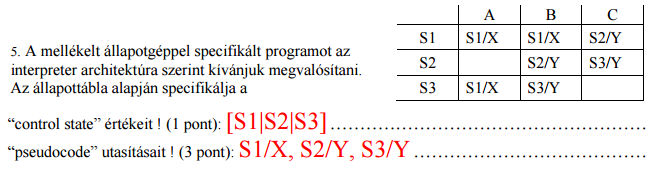
\includegraphics[scale=0.7]{img/table19}
		\end{center}

	\item Az interpreter architektúra melyik komponensének feleltethető meg egy állapottábla? (2 pont)

		 Pseudocode

	\item Az alábbi ábrán három UML2 mdoell elemet megjelöltünk. Adja meg elemenként hogy az melyik UML2 meta-modell elem példánya! (3 pont)

		\begin{center}
			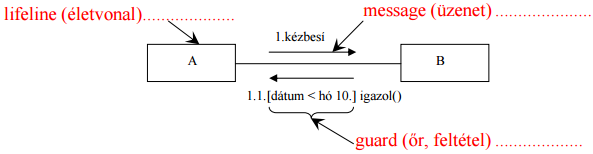
\includegraphics[scale=0.7]{img/table20}
		\end{center}

	\item Társítsa a folyamatokat a fogalmakkal

		\begin{center}
			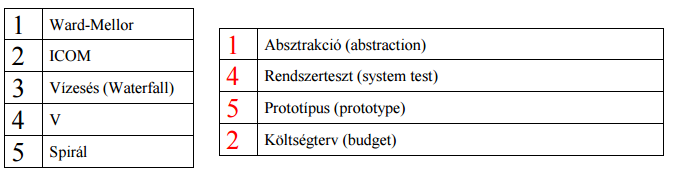
\includegraphics[scale=0.7]{img/table21}
		\end{center}

	\item Kockázatelemzés (risk analysis) során minden kockázathoz hozzárendeljük (4 pont)

		probability, seriusness (effect)

	\item Adja meg, hogy helyesek-e a következő adatfolyamábra illetve context diagram részletek !( 6 pont)

		\begin{center}
			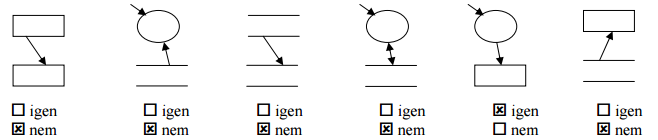
\includegraphics[scale=0.7]{img/table23}
		\end{center}


	\end{enumerate}
